\documentclass[a4paper,10pt]{article}

%Packages
\usepackage{graphicx}
\usepackage{grffile}
\usepackage{color}
\usepackage[utf8]{inputenc}

\title{Instruction manual for PowerCloud}
\author{Marc Antel, 12026973\\ Brandon Wardley, 29005150\\ Stuart Andrews, 12153983\\ Mothusi Masibi, 12004589}
\date{\today}

\begin{document}
	\maketitle
	\newpage
	\section{Compiling and Installing from Source Code}
	\subsection{Pre-requisites}
	\textbf{Software}
	Before proceeding please ensure you have the following software installed on your system:
	\begin{itemize}
		\item NodeJS and NPM
		\item Bower
		\item Gulp
		\item Particle Dev
		\item Java 8
		\item Maven
	\end{itemize}
	
	\textbf{Hardware}
	\begin{itemize}
		\item A Particle Photon.
		\item A computer with internet access which does not block incoming and outgoing connections on port 1883 and 80.
	\end{itemize}
	
	\subsection{Firmware}
	Compile and flash the photon with the following commands, please take note 
	that if you run the application server on a local machine, retrieve the IP 
	address and insert it into the firmware's code as shown below.\\
	
	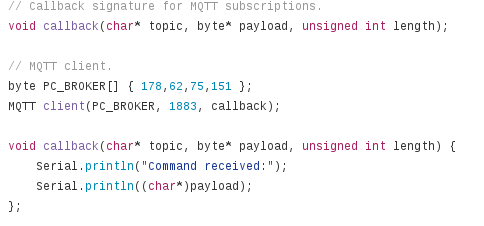
\includegraphics[scale=0.5]{images/firmware.png}
	
	Follow the instructions here in order to compile the firmware using Particle 
	Dev.
	\\
	\begin{itemize}
		\item Open the firmware using Particle Dev.
		\item Click on "\textit{Compile using Partcicle Cloud}".
		\item Select the device to flash.
		\item Click on "\textit{flash device}".
	\end{itemize}
	
	\textit{If you run into errors, please see the troubleshooting guide at the end of this document.}
	
	\subsection{Application Server}
	Currently, the \textit{application-server} branch hosts the source code for 
	the Application Server. It needs to be compiled using maven and run on a 
	device which doesn't block incoming and outgoing connections on port 1883.\\
	
	\textbf{Compiling the Application Server}\\
	Download the sources from GitHub and compile:\\
	
	\begin{itemize}
		\item \textit{\$ mvn package}
	\end{itemize}		
	
	\textit{If you run into errors, please see the troubleshooting guide at the end of this document.}
	\newpage
	\subsection{Web Application}
	
	\newpage
	\section{Starting PowerCloud}
	\subsection{Firmware}
	Once the firmware has been compiled and the binary file produced. Flash the photon with the following command:
	
	\begin{itemize}
		\item \textit{particle serial flash Photon Name *.ino}
	\end{itemize}
	
	\subsection{Application Server}
	Once the application server has been compiled, change your directory to IllusionSolutions/test/, run the application server using the following command
	
	\begin{itemize}
		\item \textit{java -jar applicationServer-*.jar}
	\end{itemize}
	
	\subsection{Web Application}
	To start the PowerCloud Web application open the console.
	
	\begin{itemize}
		\item \textit{npm install}
		\item \textit{bower install}
		\item \textit{gulp serve}
	\end{itemize}
	
	The web application should now be available on \textbf{http://localhost:9000/}
	
	\begin{figure}[H]
		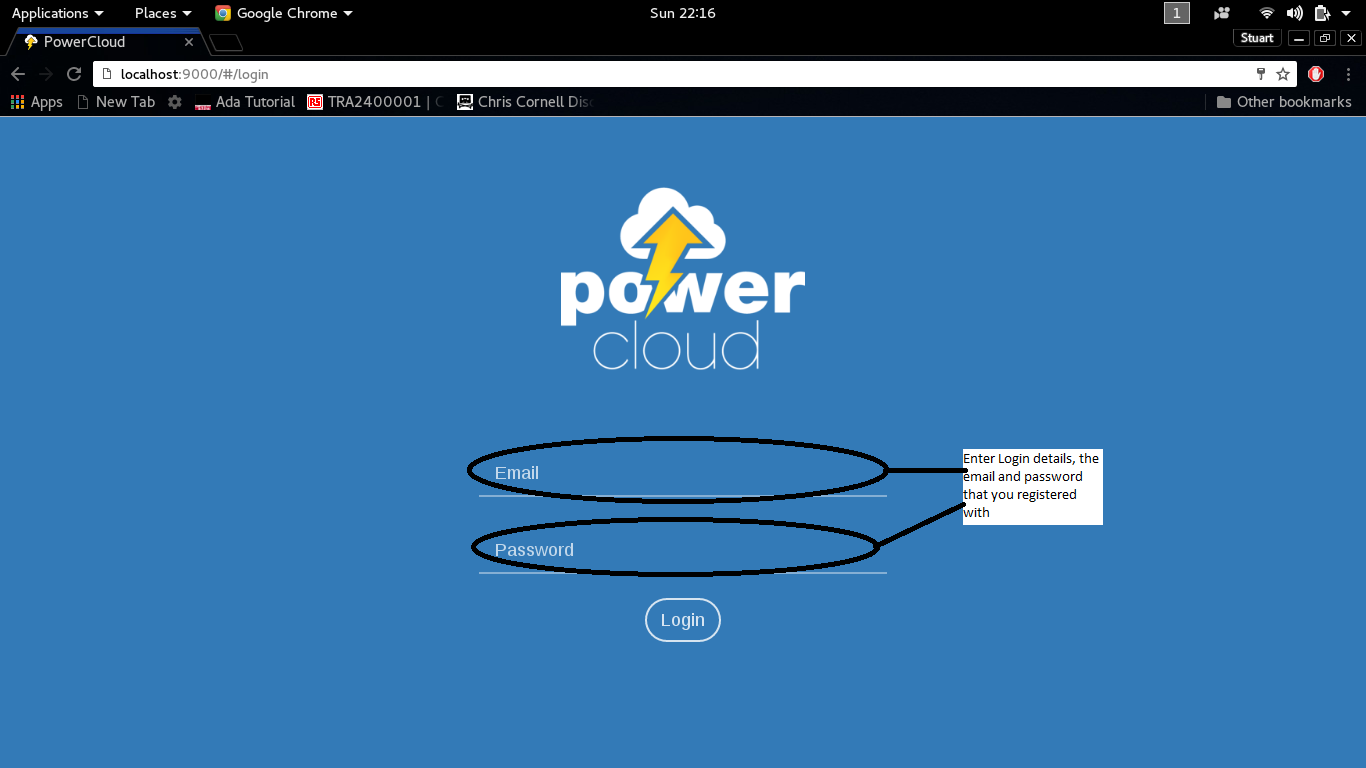
\includegraphics[scale=0.3]{images/login.png}
	\end{figure}
	
	\begin{figure}[H]
		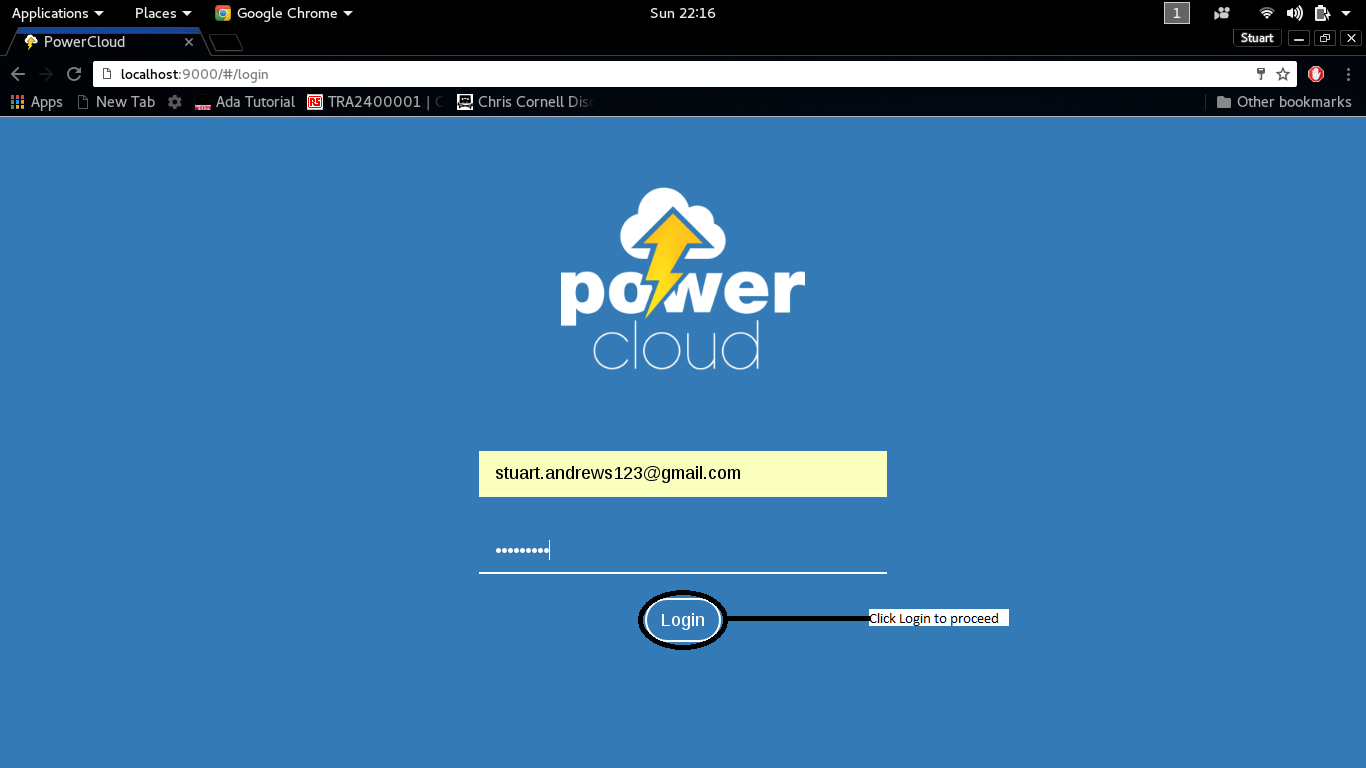
\includegraphics[scale=0.3]{images/login2.png}
	\end{figure}
	
	\begin{figure}[H]
		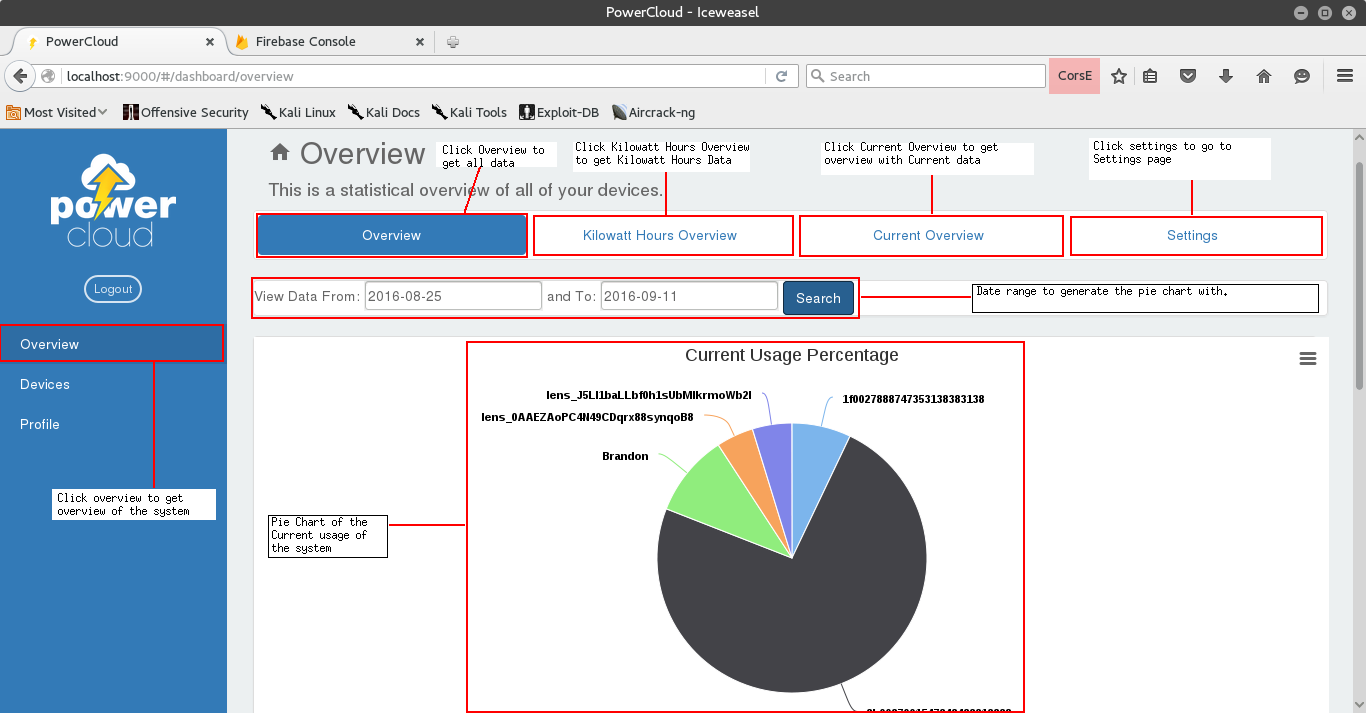
\includegraphics[scale=0.3]{images/Overview.png}
	\end{figure}
	
	\begin{figure}[H]
		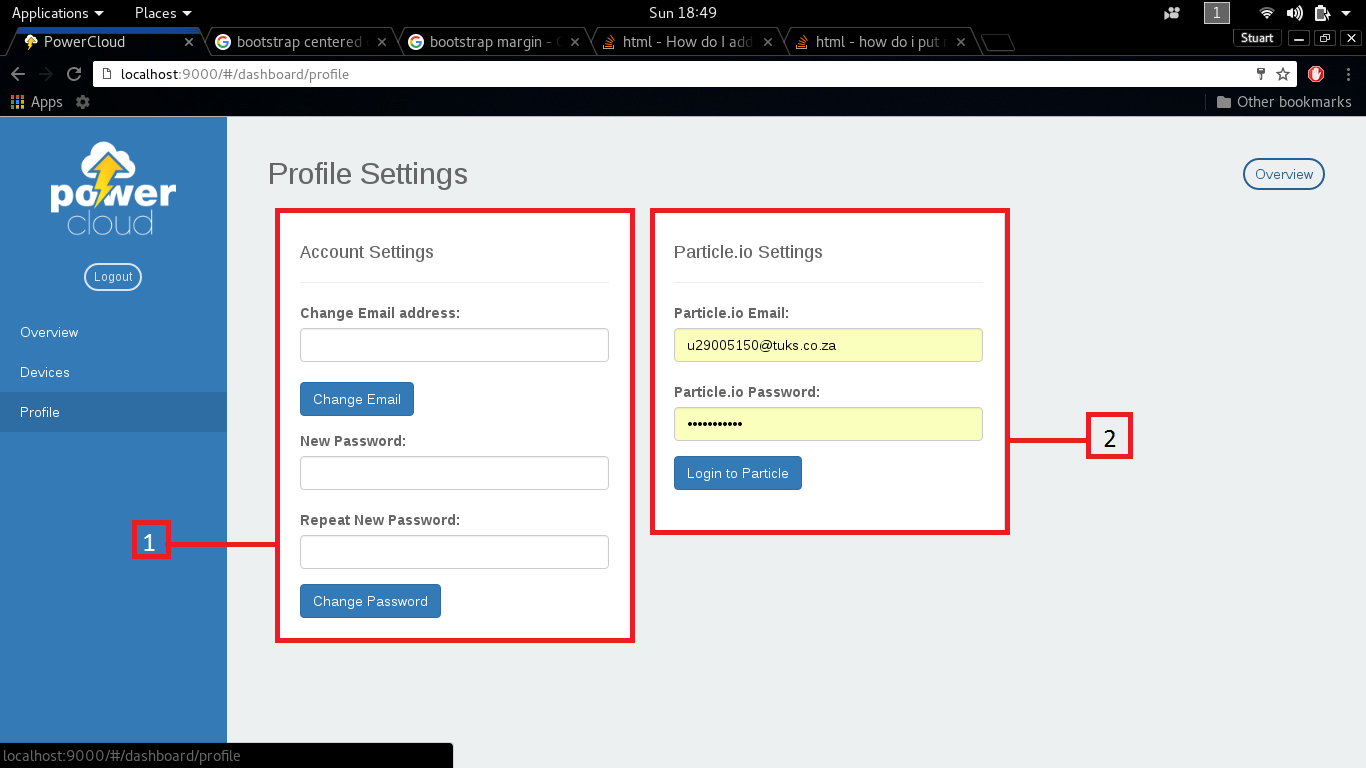
\includegraphics[scale=0.3]{images/profile.png}
	\end{figure}
	
	\begin{figure}[H]
		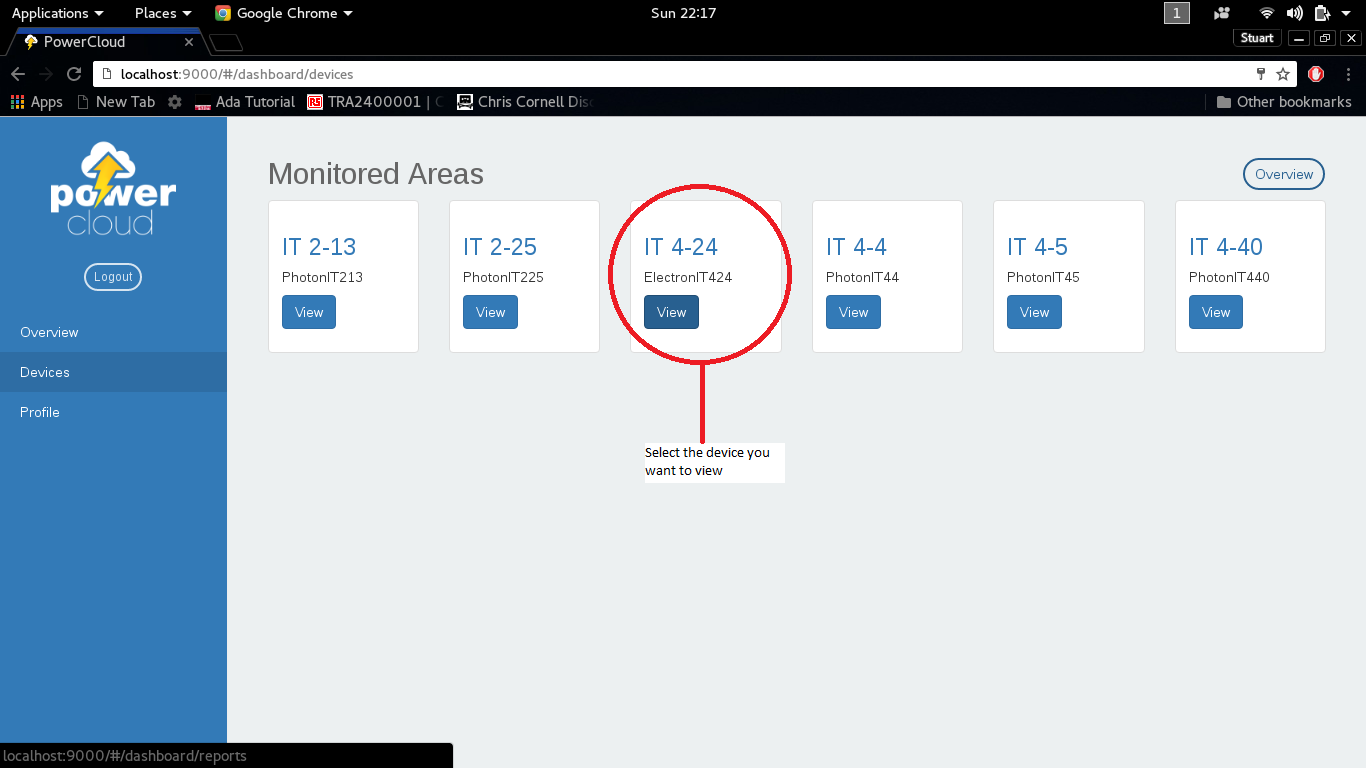
\includegraphics[scale=0.3]{images/view.png}
	\end{figure}
	
	\begin{figure}[H]
		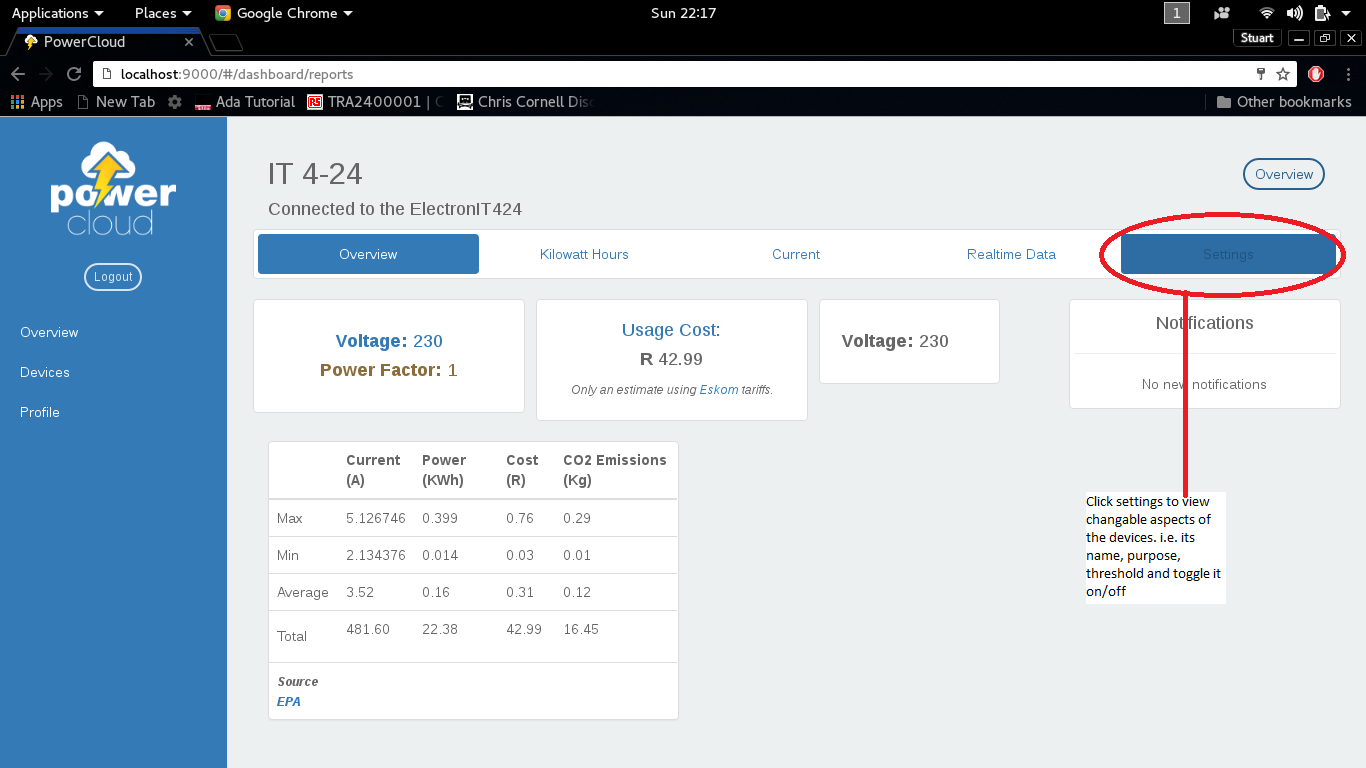
\includegraphics[scale=0.3]{images/settings1.png}
	\end{figure}
	
	\begin{figure}[H]
		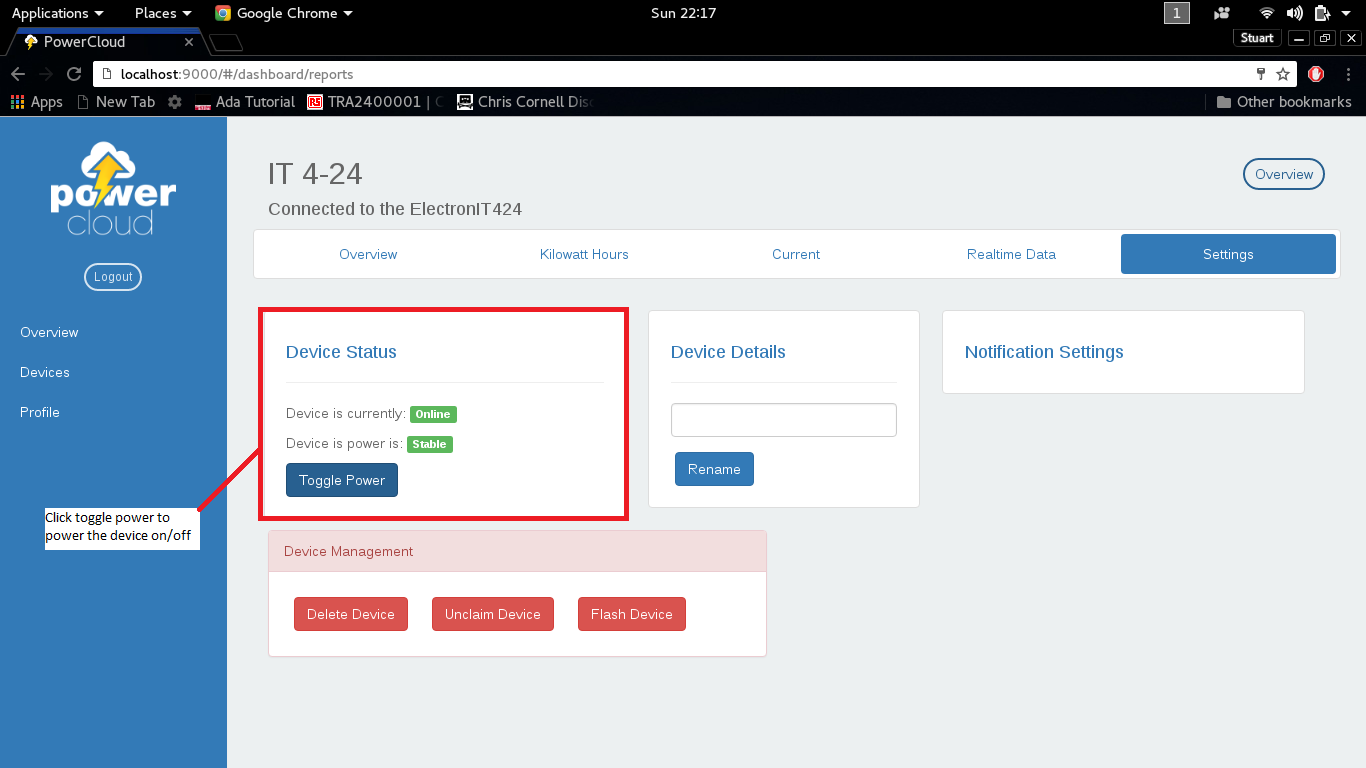
\includegraphics[scale=0.3]{images/settings.png}
	\end{figure}
	
	\newpage
	\section{Troubleshooting}
	\textbf{I am getting errors when trying to install through the console.}
	\begin{itemize}
		\item Try using sudo before the command. Example: sudo npm install particle-cli
	\end{itemize}
	
	\textbf{The Web Application won't run and is giving errors when executing the gulp serve command.} 
	\begin{itemize}
		\item Make sure you've run npm install and bower install.
		\item Make sure you're in the correct directory where the web application is located.
	\end{itemize}
\end{document}
